\begin{frame}
	\frametitle{Das Klimasystem - Zusammenfassung}

	\begin{columns}
		\column{0.3\linewidth}
			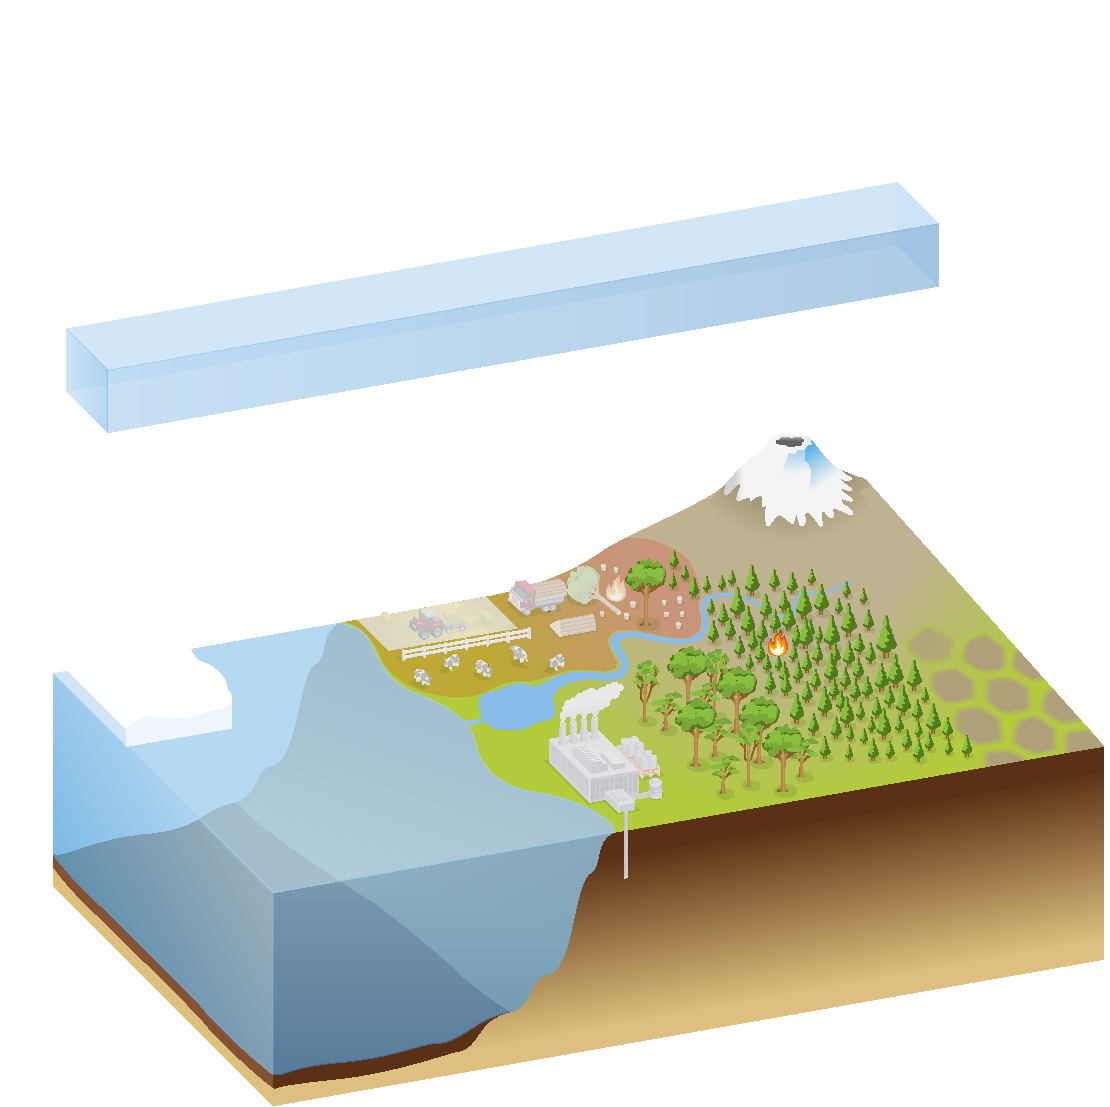
\includegraphics[trim={1cm 0cm 0cm 3cm}, clip, width=0.9\linewidth]{%
					bilder/climate_components/global_climate_components_spheres_ex_human.pdf}
		\column{0.7\linewidth}
			\begin{itemize}
				\item Das Klimasystem Erde besteht aus verschiedenen Komponenten.
				\item Das Verständnis dieser Komponenten erfordert Wissen in vielen Bereichen: Physik, Chemie, Biologie, Geologie u. a.
				\item Es treten zwischen allen Teilen zahlreiche Wechselwirkungen auf.
				\item Einzelne Komponenten reagieren auf Zeitskalen von Minuten bis hin zu Jahrmillionen.
			\end{itemize}
		\end{columns}
		\begin{columns}
			\column{0.7\linewidth}
			\begin{itemize}
				\item Klimamodelle versuchen die Erde ganzheitlich zu erfassen.
				\item Die Modelle sind sehr komplex, können aber nie alles abbilden.
				\begin{itemize}
					\item So viel wie nötig, so wenig wie möglich
					\item Modelle verbessern sich mit der Zeit und Technik
					\item Bessere Modelle helfen menschlichen Einfluss auf das Klima genauer zu bestimmen
					\item[$\rightarrow$] Grundlegende Aussagen ändern sich wenig
				\end{itemize}
			\end{itemize}
			\column{0.3\linewidth}
				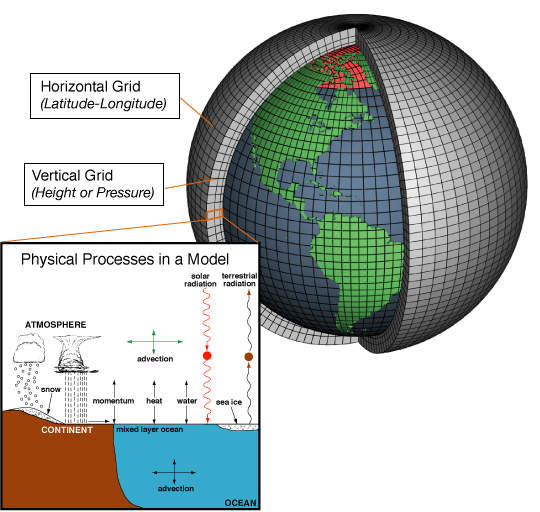
\includegraphics[width=0.9\linewidth]{bilder/AtmosphericModelSchematic.png}
		\end{columns}

	\note{
	\begin{itemize}
		\item[] Abbildung mit allen zuvor erklärten (größeren) Klimakomponenten
		\item[] viele kleinere Bereiche wie die Böden oder bestimmte Stoffkreisläufe sind ebenfalls wichtig
		\item[] es ist ein sehr komplexes System, an dem in vielen Stellen Änderungen und Wechselwirkungen auftreten (z.B. Eis-Albedo)
		\item[] also: komplexes System, mit komplexen Zusammenhängen
		\item[] in einzelnen Bereichen wie der Wolkenbildung sind noch Forschungsfragen offen
		\item[] (wir wollen Klarheit reinbringen, damit Lösungen eher im Kontext betrachtet werden können)
		\item[] (Eine Lösung kann nämlich Rückkopplungseffekte in anderen Bereichen erzeugen)
	\end{itemize}
	}
\end{frame}
